\documentclass[margin = 1cm]{standalone}
\usepackage{tikz}
\usepackage{amssymb}
\usetikzlibrary{shapes.geometric,arrows.meta}
\tikzset{one/.style={draw = #1,minimum width = 5em,fill = #1!20,align = center,inner xsep = .5cm,inner ysep = .3cm},
arrow/.style = {-{Triangle[scale = 1]},thick}}

\begin{document}
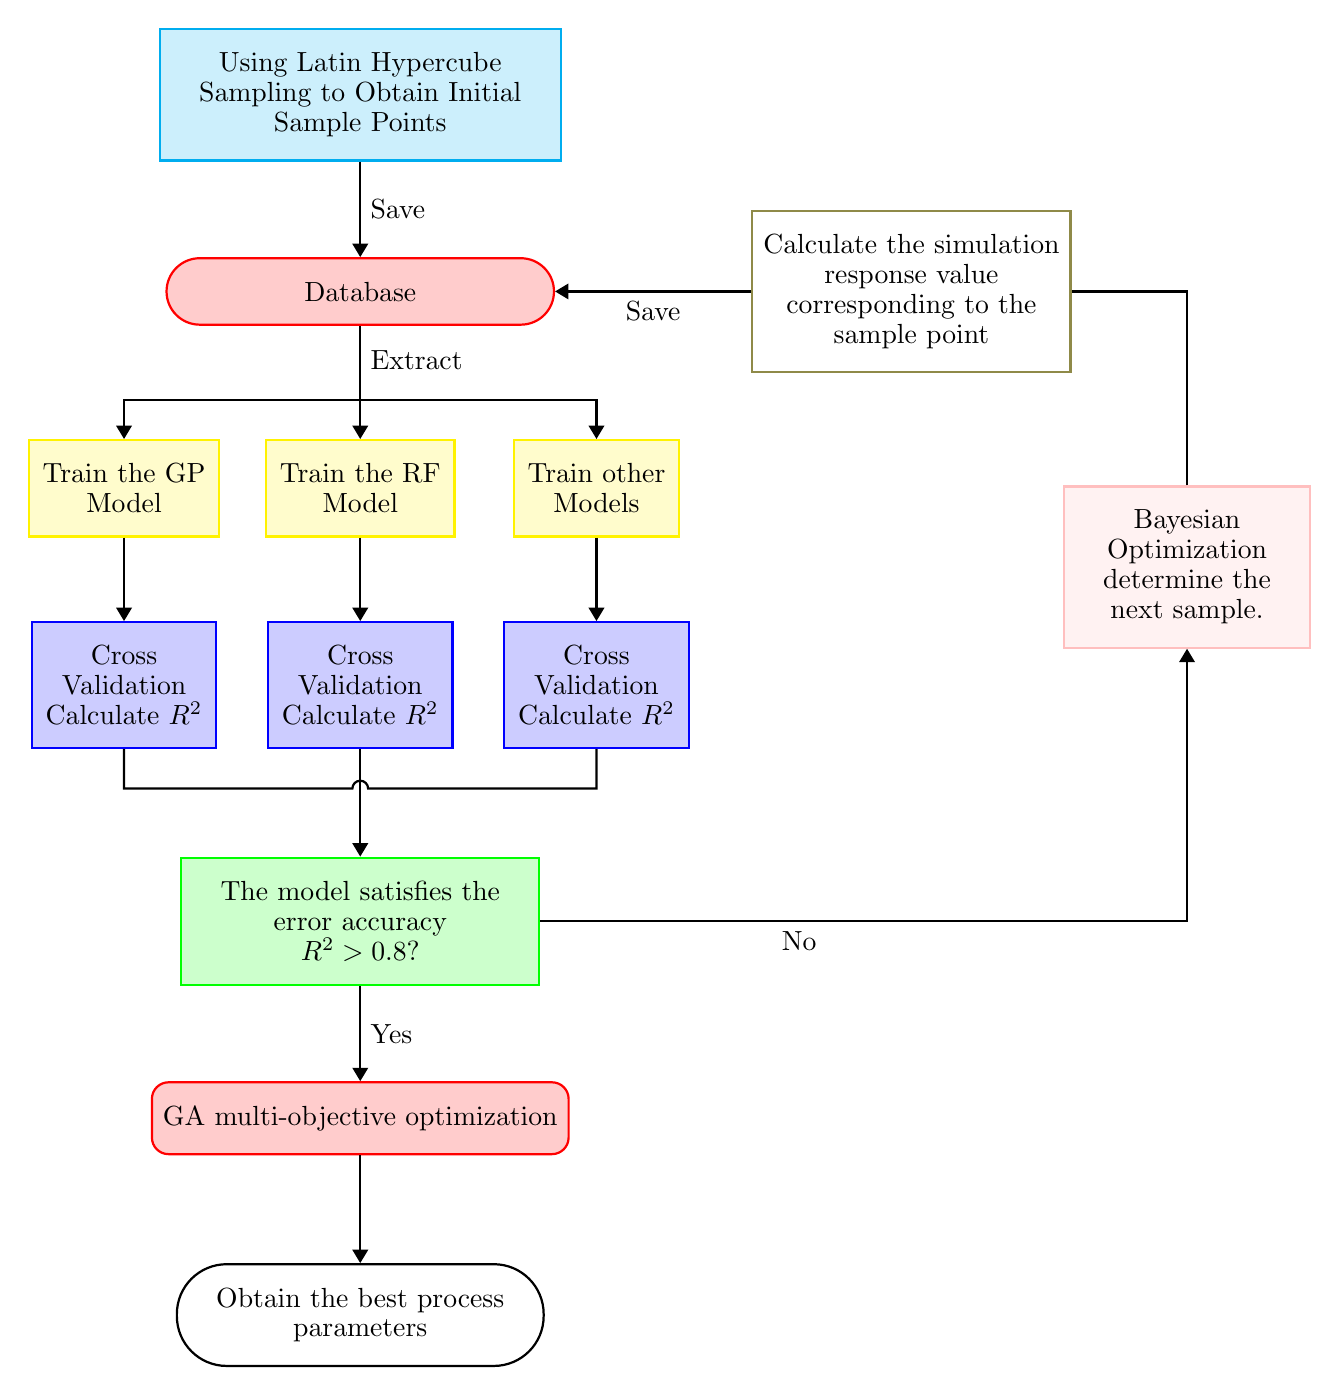
\begin{tikzpicture}[thick]
\linespread{.9}
\node[one = cyan] (a) at (0,0) {Using Latin Hypercube \\ Sampling to Obtain Initial \\ Sample Points};
\node[one = red,minimum width = 14em,rounded corners = 12pt] (b) at (0,-2.5) {Database};

\node[one = yellow,inner xsep = 5pt] (c) at (-3,-5) {Train the GP \\ Model};
\node[one = yellow,inner xsep = 5pt] (d) at (0,-5) {Train the RF \\ Model};
\node[one = yellow,inner xsep = 5pt] (e) at (3,-5) {Train other \\ Models};

\node[one = blue,inner xsep = 5pt] (f) at (-3,-7.5) {Cross \\ Validation \\ Calculate $R^2$};
\node[one = blue,inner xsep = 5pt] (g) at (0,-7.5) {Cross \\ Validation \\ Calculate $R^2$};
\node[one = blue,inner xsep = 5pt] (h) at (3,-7.5) {Cross \\ Validation \\ Calculate $R^2$};

\node[one = green] (i) at (0,-10.5) {The model satisfies the \\ error accuracy \\ $R^2>0.8?$};

\node[one = red, thick, rounded corners = 6pt,inner xsep = 4pt] (j) at (0,-13) {GA multi-objective optimization};

\node[one = black, rounded corners = 18pt,fill = white] (k) at (0,-15.5) {Obtain the best process \\ parameters};

\node[one = pink] (l) at (10.5,-6) {Bayesian \\ Optimization \\ determine the \\ next sample.};

\node[one = yellow!50!black,thick,fill = white,inner xsep = 4pt] (m) at (7,-2.5) {Calculate the simulation \\response value \\ corresponding to the \\ sample point};

\draw[arrow] (a) -- (b)node[pos = .5,right]{Save};
\draw[arrow] (b) -- (d)node[pos = .3,right]{Extract};
\draw[Triangle-Triangle] (c.north) -- ++(0,.5cm) -| (e);
\draw[arrow] (c) -- (f);
\draw[arrow] (d) -- (g);
\draw[arrow] (e) -- (h);

\draw[arrow] (g) -- (i);
\draw[arrow] (i) -- (j)node[pos = .5,right]{Yes};
\draw[arrow] (j) -- (k);

\draw[] (f.south) -- ++ (0,-.5cm) -- ++ (2.9,0) arc[start angle = 180,end angle = 0, radius = .1cm] -| (h);

\draw[arrow] (i) -| (l)node[pos = .2,below]{No};
\draw[] (l) |- (m);
\draw[arrow] (m) -- (b)node[pos = .5,below]{Save};
\end{tikzpicture}
\end{document}